\section{Activity Structure}
\label{implementation:activity_structure}
\begin{figure}[h!]
	\centering
	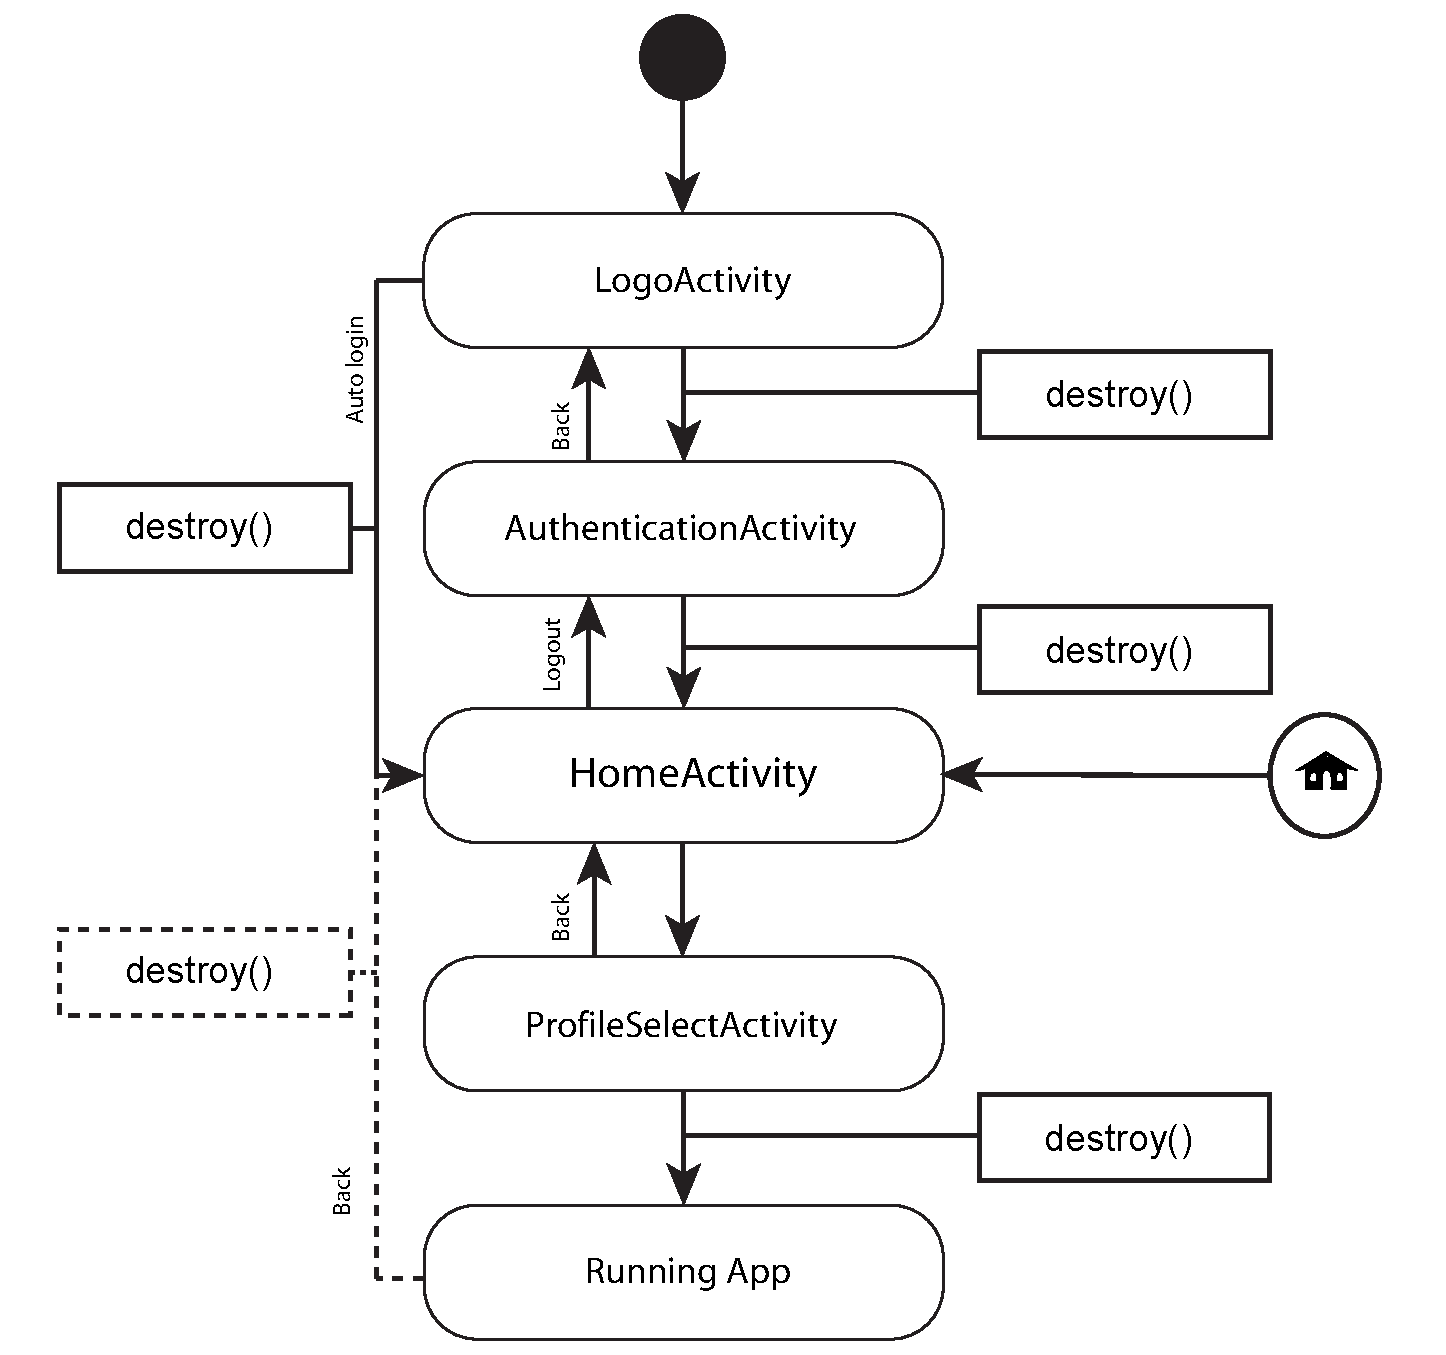
\includegraphics[width=1\textwidth]{gfx/activityDiagram.pdf}
	\caption{Activity diagram of the launcher}
	\label{fig:activity_diagram}
\end{figure}

\autoref{fig:activity_diagram} shows the activity structure of the \giraf[] launcher. 
Every path with a \verb+destroy()+ box on it gets the activity starting the path destroyed.
Pressing the back button will also the destroy the activity it was pressed, and the \activity{HomeAcitivity}, which implements the app management functionality, is also destroyed on log out.
Every time the user is outside the launcher and hits the home button, they will end up in the \activity{HomeActivity}, if the \giraf[] launcher is set to the default launcher.
Note that this is a feature in Android. 
The dotted section symbolizes that the launcher does not have any control in this area, as it belongs to the launched app.

When the launcher is started, the user is presented with the \activity{LogoActivity}, which implements the initialization functionality, from which they will be redirected to the \activity{AuthenticationActivity}, which implements the authentication functionality, to perform the authentication. 
In this process, the \activity{LogoActivity} is destroyed.
If the user authenticates, the \activity{HomeActivity} is called. 
If an app is clicked in the \activity{HomeActivity}, the user will be presented with the \activity{ProfileSelectActivity}, which implements the profile selection functionality, and must choose a child before they can start this app.